\chapter{Fourier transform as measurement of radial velocity}
\label{\thechapter}
\label{ch:Methods}
\addcontentsline{lof}{chapter}{\protect\numberline{\arabic{chapter}} {\nameref{\thechapter}}}

%----------------------------------------------------------------------------------------

\rule{\textwidth}{1.6pt}
\minitoc
\clearpage

%----------------------------------------------------------------------------------------

This chapter will introduce a new method to measure the radial velocity. We will study, in Fourier transform, 
the features of a signal shift from time domain to frequency domain. The results will be applied to measuring non-deformed
spectral line shifts. We will then extend the study to measuring the apparent radial velocity shift 
due to line profile deformation. 


\section{Fourier transform as measurement of line shift}
\label{\thesection}
\label{ch:FT_line_shift}


\subsection{Translation property of Fourier transform}
Translation is also known as time shifting, as Fourier transform usually deals with time sequence signals. 
In this chapter, we use time domain and frequency domain to differentiate the signal before and after Fourier transform,
regardless of the nature of the signal. 

Let $h(x)$ be a signal $f(x)$ delayed (or shifted) by $x_0$:
\begin{equation}
	h(x) = f(x-x_0).
\label{eq:FT1}
\end{equation}
In the frequency domain, we have 
\begin{equation}
	\hat{h}(\xi) = e^{-2 \pi ix_0 \xi} \hat{f}(\xi),
\label{eq:FT2}
\end{equation}
where the circumflex denotes Fourier transform of a function. This formula shows that $\hat{h}(\xi)$ and $\hat{f}(\xi)$ 
differ by a frequency dependent phase angle 
\begin{equation}
	\Delta \phi(\xi) = -2 \pi x_0 \xi
\label{eq:PhaseShift}
\end{equation}
while the power spectral density remains the same (as $\mid e^{-2 \pi ix_0 \xi}\mid ^2 = 1$).


\subsection{Intuitive explanation}

Although the translation property of Fourier transform can be mathematically proven, I provide a more 
intuitive explanation in the following. 

By definition
\begin{equation}
	\hat{f}(\xi) = \int_{-\infty}^{\infty} f(x) e^{-2 \pi ix \xi} dx, 
\label{eq:FT3}
\end{equation}
Fourier transform decomposes the function $f(x)$ into frequency representations $\hat{f}(\xi)$, such that the function itself can be  
expressed as the sum of \textit{all} orthogonal basis $e^{2 \pi ix \xi}$, which is also known as the inverse Fourier transform:
\begin{equation}
	f(x) = \int_{-\infty}^{\infty} \hat{f}(\xi) e^{2 \pi ix \xi} d\xi. 
\end{equation}

Note that shifting $f(x)$ by $x_0$ is equivalent to shifting \textit{all} the orthogonal basis by $x_0$, which becomes 
$e^{2 \pi i(x-x_0) \xi}$. This is how the extra term $e^{-2 \pi ix_0 \xi}$ comes along -- it contributes to the phase difference 
\footnote{For a simplified vision bridging a shift of the signal in the time domain and a phase difference in the frequency domain, imagine any real continuous function is a sum of sines and cosines. Changing the phase angle in the sines and cosines results in shifts in the function.}.

The fact that the power spectrum density remains the same can also be viewed intuitively -- shifting the signal as a whole 
doesn't add or remove any frequency information. In other words, the composition of the signal doesn't change. 


\subsection{How to use}

From Eq.~\ref{eq:PhaseShift}, we could see that the phase shift $\Delta \phi(\xi)$ is proportional to the frequency $\xi$
with the constant gradient
\begin{equation}
	\text{slope} = \dv{(\Delta \phi)}{\xi} = -2 \pi x_0
\label{eq:gradient}
\end{equation}
In practice, obtaining the slope is as easy as fitting the measured $\Delta \phi(\xi)$ and $\xi$ 
with linear regression model (Fig.~\ref{fig:FT}). Therefore, the shift can be calculated as 
\begin{equation}
	x_0 = -\frac{\text{slope}}{2 \pi}
\label{eq:line_shift}
\end{equation}

Analogous to the definition of power spectral density, we call $\phi(\xi)$ the phase spectral density and hence $\Delta \phi(\xi)$ the differential phase spectral density. 

%-------------
\begin{figure}[tbp]
\centering
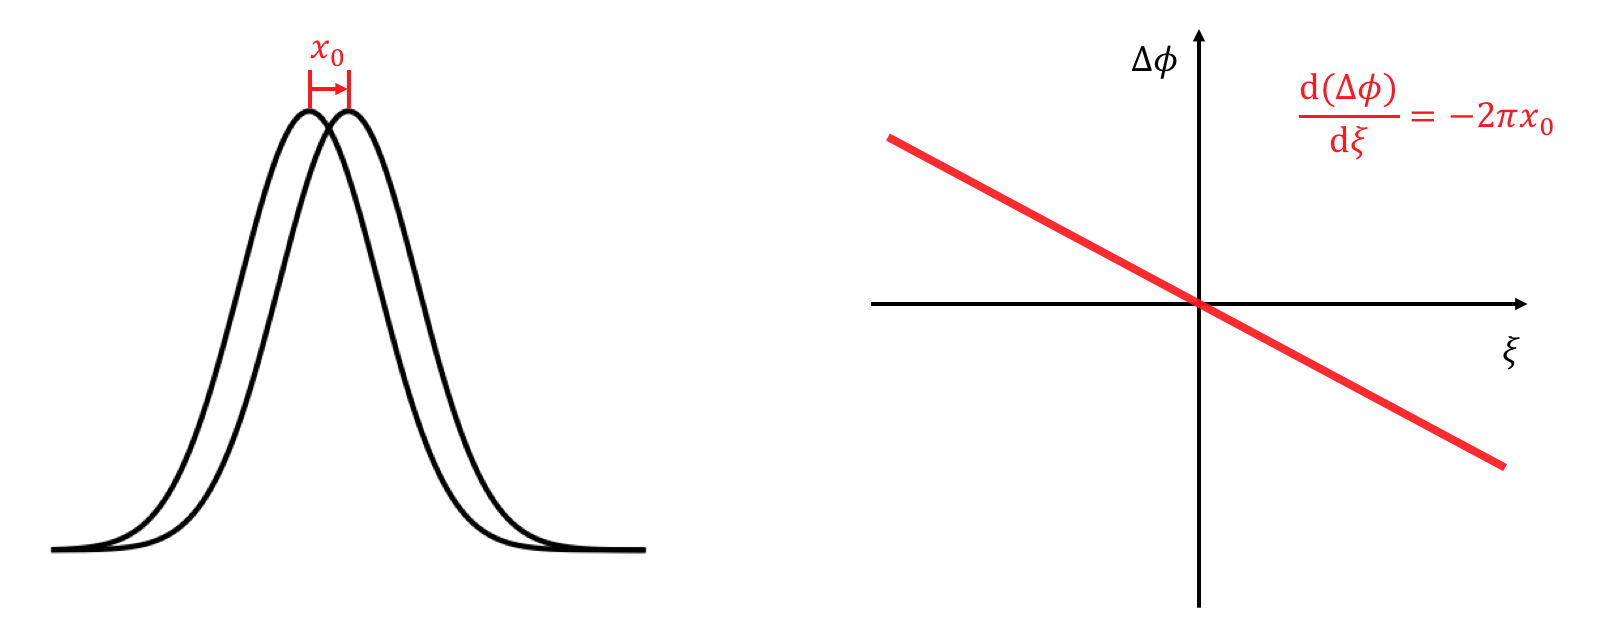
\includegraphics[width = 0.99 \linewidth]
{./Figures/Methods/FT.png}
\caption[Translation property of Fourier transform]
{The left panel shows a signal (or a spectral line profile in the following context) shifted by an amount $x_0$. 
The right panel is the differential phase spectral density diagram (i.e. differential phase spectrum). 
The model shows a perfectly linear correlation 
between $\Delta \phi(\xi)$ and $\xi$ with the constant slope $-2 \pi x_0$.}
\label{fig:FT}
\end{figure} 
%-------------

\paragraph{Concluding remarks}
Fourier transform bridges the signal shift (or delay) in the time domain and the phase shift in the frequency domain,
and hence the phase shift can be used to estimate signal shift by Fourier transform.

%----------------------------------------------------------------------------------------	

\subsection{Sanity check}

We will perform a sanity check to see if we could correctly recover the shifts of a line profile  
by analysing the phase shift through Fourier transform. 

First of all, we generate a spectral line profile based on the cross-correlation function of observed HARPS spectrum
with the software SOAP 2.0. A tiny amount of noise (S/N=10,000) has been injected in the line profiles. 
We then apply 100 radial velocity shifts evenly spaced between 0 and 10 m/s (Fig.~\ref{fig:line_profiles12}). 
The Fourier transform of the 100 spectral line profiles divides the information into two parts: 
(1) the power spectra (Fig.~\ref{fig:power_spectrum}) and (2) the phase spectra, from which we obtain the 
differential phase spectra relative to the non-shifted line profile (Fig.~\ref{fig:dps}). 
We notice that most of the information are concentrated in the lower frequency range in the power spectrum, and 
as expected, the differential phase spectra are linear by eye \footnote{The slight deviation from linearity may come from
the noise that we injected.}. The slopes of the differential phase spectra indicate the amount of shifts relative to 
the non-shifted line profile. At last we calculate the radial velocity shifts using two methods: 
(1) $RV_\text{FT}$ from Eq.~\ref{eq:line_shift} and 
(2) $RV_\text{Gaussian}$ traditionally the line centroid by fitting a Gaussian profile, both compared with 
the input line shift (Fig.~\ref{fig:rv_recovery}). The root mean square of the residual
are $rms_\text{FT} = 0.13$ m/s and $rms_\text{Gaussian} = 0.09$ m/s respectively, indicating 
very consistent radial velocities. Note that $rms_\text{FT}$ is slightly larger than $rms_\text{Gaussian}$.
This is because we only use part of the information from the line profile -- the lower frequency section of the 
differential phase spectra. In fact, higher frequency range becomes useless 
as the interpretation of Fourier transform in high frequencies is dominated by noise and does not represent the 
intrinsic shift of the line profile any more. As a result, linearity of phase spectrum breaks down in higher frequencies. 
The range of ``useful" frequencies will depend on the amount of noise (i.e. S/N). 

%-------------
\begin{figure}[tbp]
    \begin{subfigure}[b]{0.49\textwidth}
        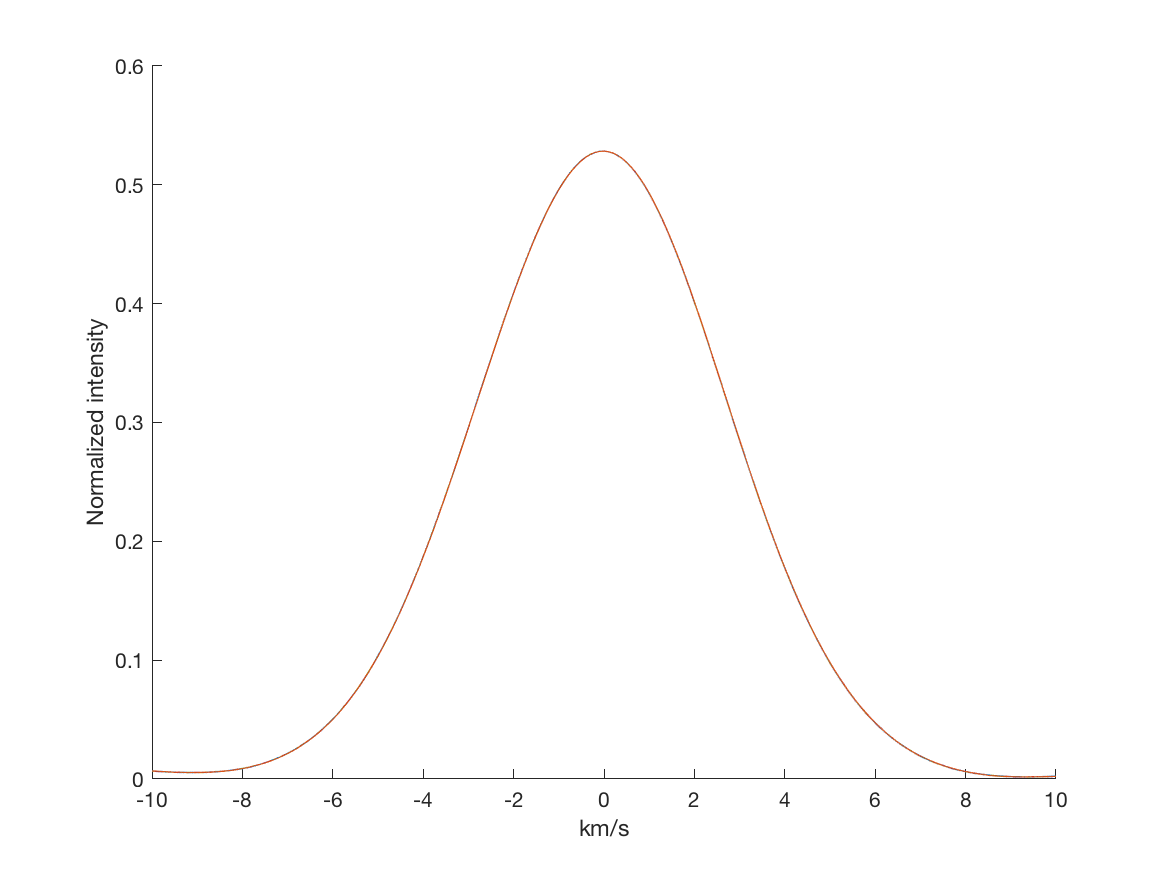
\includegraphics[width=\textwidth]{./Figures/Methods/1-Line_Profile.png}
        \caption{Line profile (stacked)}
        \label{fig:line_profiles}
    \end{subfigure}
	~
    \begin{subfigure}[b]{0.49\textwidth}
        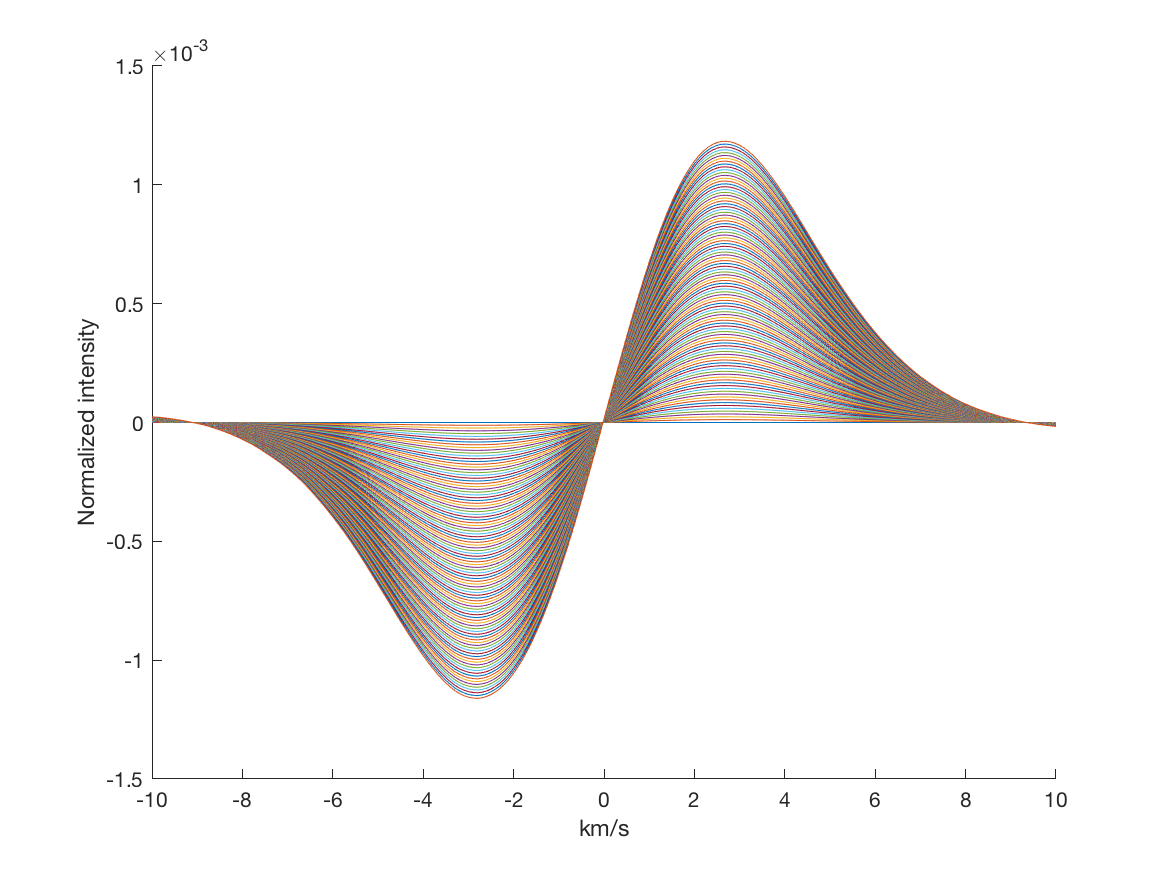
\includegraphics[width=\textwidth]{./Figures/Methods/1-Differential_line_Profile.png}
        \caption{Differential line profile}
        \label{fig:differential_line_profiles}
    \end{subfigure}	
    
    \caption[Shifted line profile]{Shifted line profile. Note that for demonstration purpose, noise is not included in  
    this differential line profile plot, otherwise the pattern of the differential will be overwhelmed by noise.}
\label{fig:line_profiles12}
\end{figure}	
%-------------
	
%-------------
\begin{figure}[tbp]	
    \begin{subfigure}[b]{0.49\textwidth}
        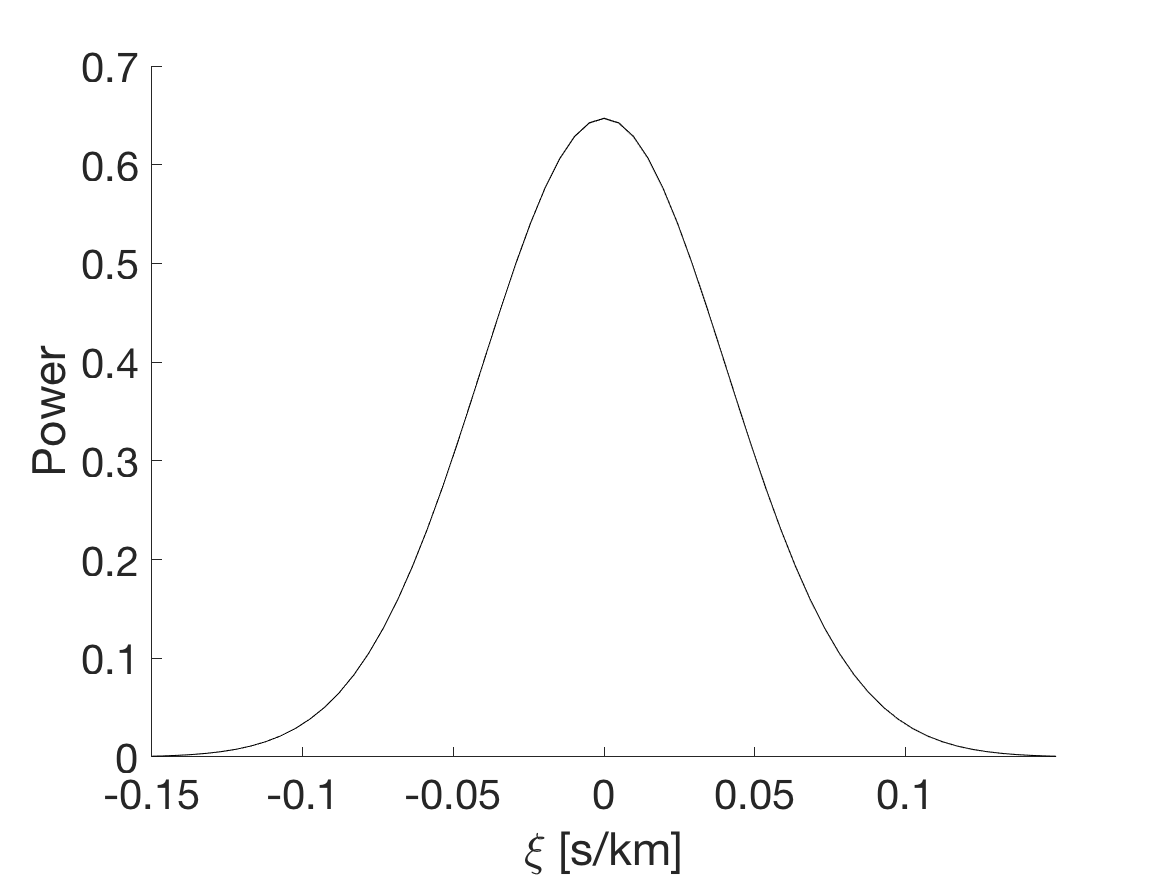
\includegraphics[width=\textwidth]{./Figures/Methods/2-FT_power.png}
        \caption{Power spectrum (stacked)}
        \label{fig:power_spectrum}
    \end{subfigure}
	~
    \begin{subfigure}[b]{0.49\textwidth}
        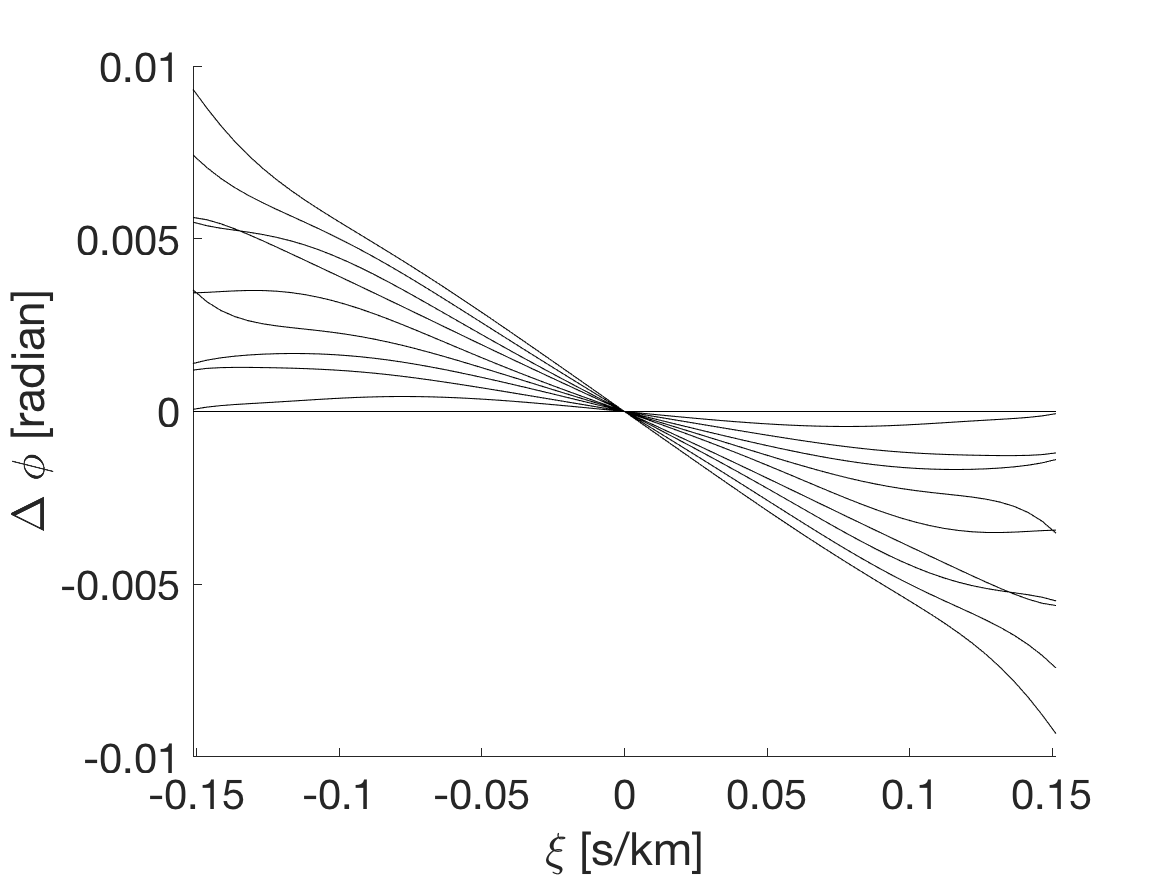
\includegraphics[width=\textwidth]{./Figures/Methods/4-Relative_phase_angle.png}
        \caption{Differential phase spectrum}
        \label{fig:dps}
    \end{subfigure}	
    
    \caption[Fourier transform of shifted line profile]{Fourier transform of shifted line profile divides the 
    information into the power spectrum and the (differential) phase spectrum. For a line shift in time domain, 
    it is translated into phase shift in frequency domain, and shows linearity in the (differential) phase spectrum.}
\label{fig:FT_process}
\end{figure}    
%-------------

%-------------
\begin{figure}[htbp]
\centering
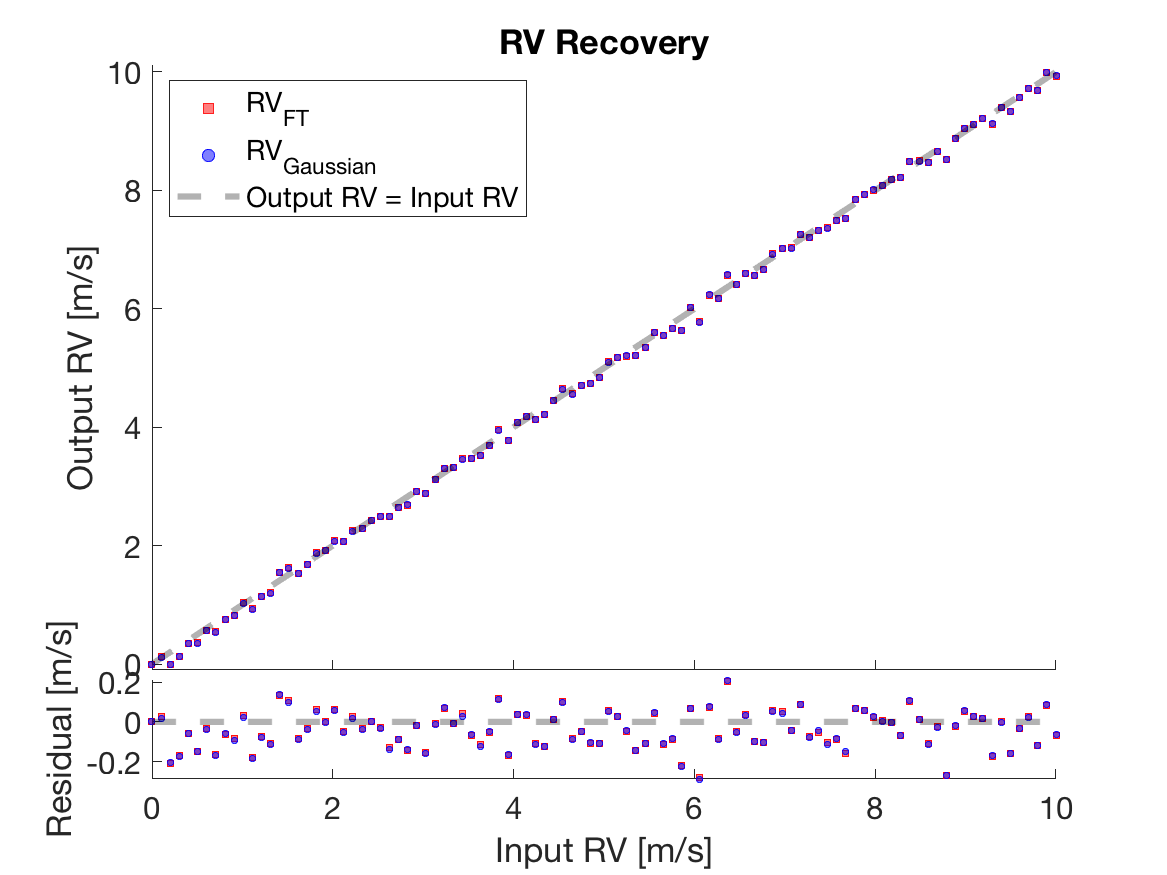
\includegraphics[width = 0.8 \linewidth]
{./Figures/Methods/5-LINE_SHIFT_ONLY.png}
\caption[Radial velocity recovery]
{Radial velocity recovery of line shifts}
\label{fig:rv_recovery}
\end{figure} 
%-------------

\paragraph{Concluding remarks}
The sanity check has passed -- we have successfully recovered the radial velocity shifts of the line profile 
by the phase shift analysis in Fourier transform. We view this method as an alternative to the traditional 
ways of obtaining the radial velocity under the circumstances where no line deformation is present. 

In a broader context, we expect this method will be applicable to measuring shifts of any pattern, and it 
can be extended to higher dimensions. In this thesis, we primarily use it to detect radial velocity shifts 
of spectral line profile. 

%----------------------------------------------------------------------------------------	

\section{Fourier transform as measurement of line deformation}
\label{\thesection}
\label{sec:FT_ld}


\subsection{Theory}
\label{sec:LD_Theory}

With this new method to detect radial velocities, we are eager to test out, its response to 
the apparent radial velocity due to spectral line deformation. In \S~\ref{ch:FT_line_shift},
the same shift $x_0$ applies to \textit{all} the basis frequencies. This is a very important premise so that 
we could make use of the linearity of the differential phase spectral density $\Delta \phi(\xi)$ (see Eq.~\ref{eq:PhaseShift}). 
In the case of line deformation due to stellar variability, $x_0$ becomes frequency dependent 
\footnote{excluding the case where the result of a line deformation is exactly the same as a line shift, as 
this becomes indistinguishable by any means}. That is to say, basis functions of different frequencies would 
shift by different amounts, resulting in shape changes (e.g. skewness) in the line profile. 
Therefore we modify the translation property of Fourier transform
by rewriting $x_0$ as $x_0(\xi)$ in Eq.~\ref{eq:PhaseShift}:
\begin{equation}
	\Delta \phi(\xi) = -2 \pi x_0(\xi) \xi.
\label{eq:PhaseShift2_LPD}
\end{equation}
As a result, the local gradient of the differential phase spectrum becomes 
\begin{equation}
	\dv{(\Delta \phi)}{\xi} = -2 \pi (x_0 + \dv{x_0}{\xi}),
\label{eq:PhaseShift3_LPD}
\end{equation}
which degenerates to Eq.~\ref{eq:gradient} when $x_0$ is a constant as in the case of line shifts.
Note that the dependency of $\xi$ has been taken out from $\Delta \phi(\xi)$ and 
$x_0(\xi)$ in writing the differential equation above. 

In principle, we could numerically solve this differential equation based on the measured local gradient d$(\Delta \phi)$/d$\xi$
to obtain $x_0(\xi)$. As a simplistic approach, if $x_0(\xi)$ changes with $\xi$ slowly within a certain frequency range,
we can make the approximations that $x_0\sim$~const and d$x_0$/d$\xi\sim0$. With this, Eq.~\ref{eq:PhaseShift3_LPD} 
converges back to Eq.~\ref{eq:gradient}.

\subsection{SOAP Simulations}
\label{sec:Simulations}


With SOAP~2.0, we inject three spots with different longitudes, latitudes and sizes (Table~\ref{table:spot_configurations}) 
and generate 100 of the cross-correlation functions of the deformed line profiles evenly sampled throughout the rotation
period of the star (Fig.~\ref{fig:line_profiles_deformation}). We then take the same approach as if we dealt with line shifts in 
\S~\ref{ch:FT_line_shift}. 

%-------------
\begin{table}[htbp]
\centering
\begin{tabular}{|c|c|c|c|}
\hline 
 & Longitude & Latitude & Size in disk area percentage\\ 
\hline 
Spot 1 & $174^\circ$ & -$14^\circ$ & 0.18\% \\ 
\hline 
Spot 2 & $288^\circ$ & $74^\circ$  & 0.40\% \\ 
\hline 
Spot 3 & $51^\circ$  & $52^\circ$  & 0.50\% \\ 
\hline 
\end{tabular} 
\caption{Spot configurations}
\label{table:spot_configurations}
\end{table}
%-------------

%-------------
\begin{figure}[tbp]
    \begin{subfigure}[b]{0.49\textwidth}
        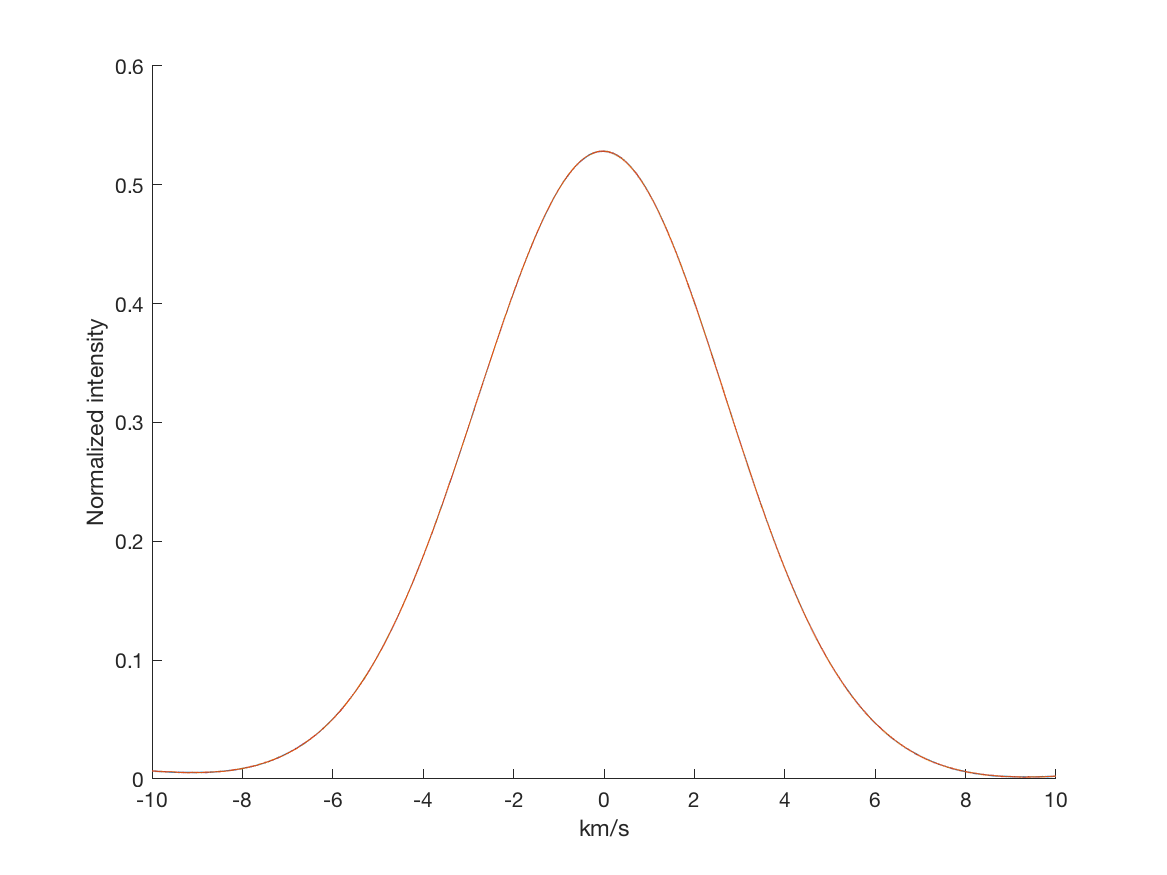
\includegraphics[width=\textwidth]{./Figures/Methods/LPD1-Line_Profile.png}
        \caption{Line profile (stacked)}
    \end{subfigure}
	~
    \begin{subfigure}[b]{0.49\textwidth}
        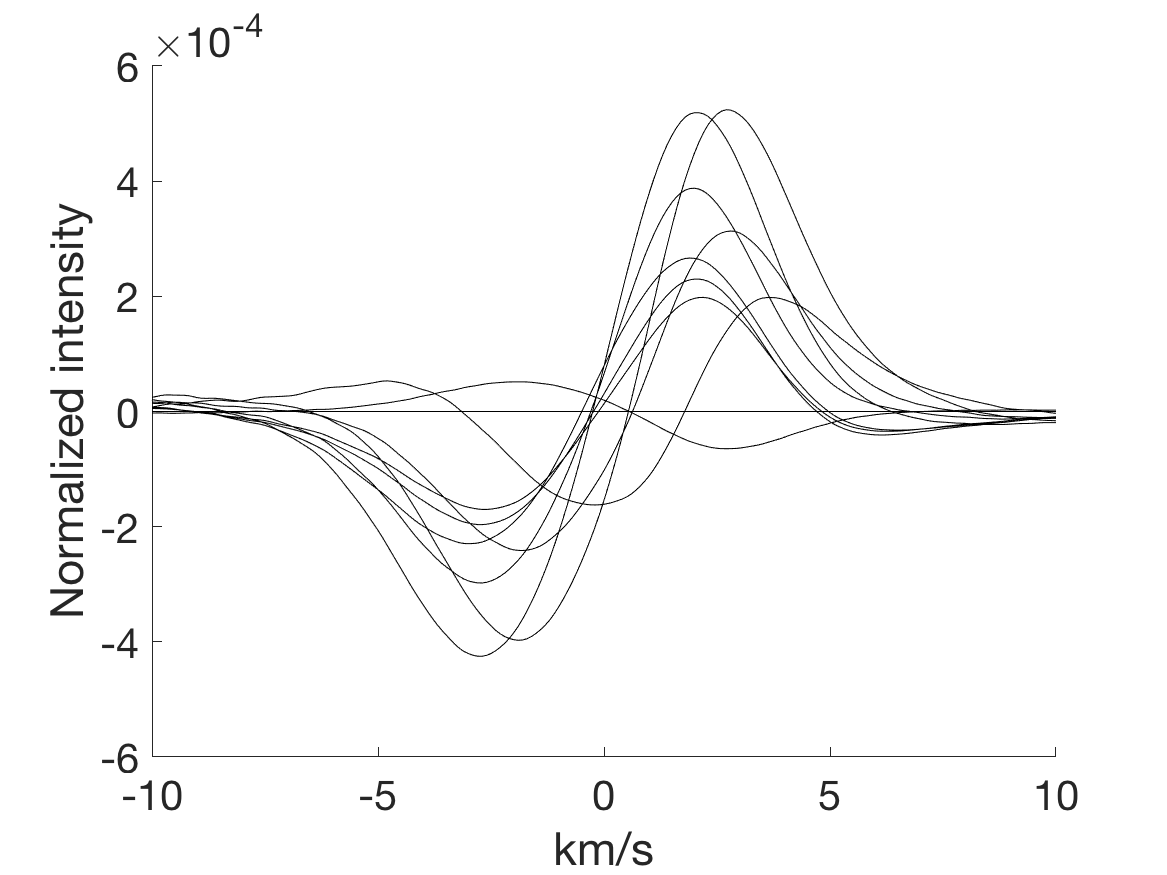
\includegraphics[width=\textwidth]{./Figures/Methods/LPD1-Differential_line_Profile.png}
        \caption{Differential line profile}
        \label{fig:ld_dlp}
    \end{subfigure}	
    
    \caption[Deformed line profile]{Deformed line profile. Note that noise is not included in  
    this differential line profile plot for the same reason.}
\label{fig:line_profiles_deformation}
\end{figure}	
%-------------

%-------------
\begin{figure}[tbp]	
    \begin{subfigure}[b]{0.49\textwidth}
        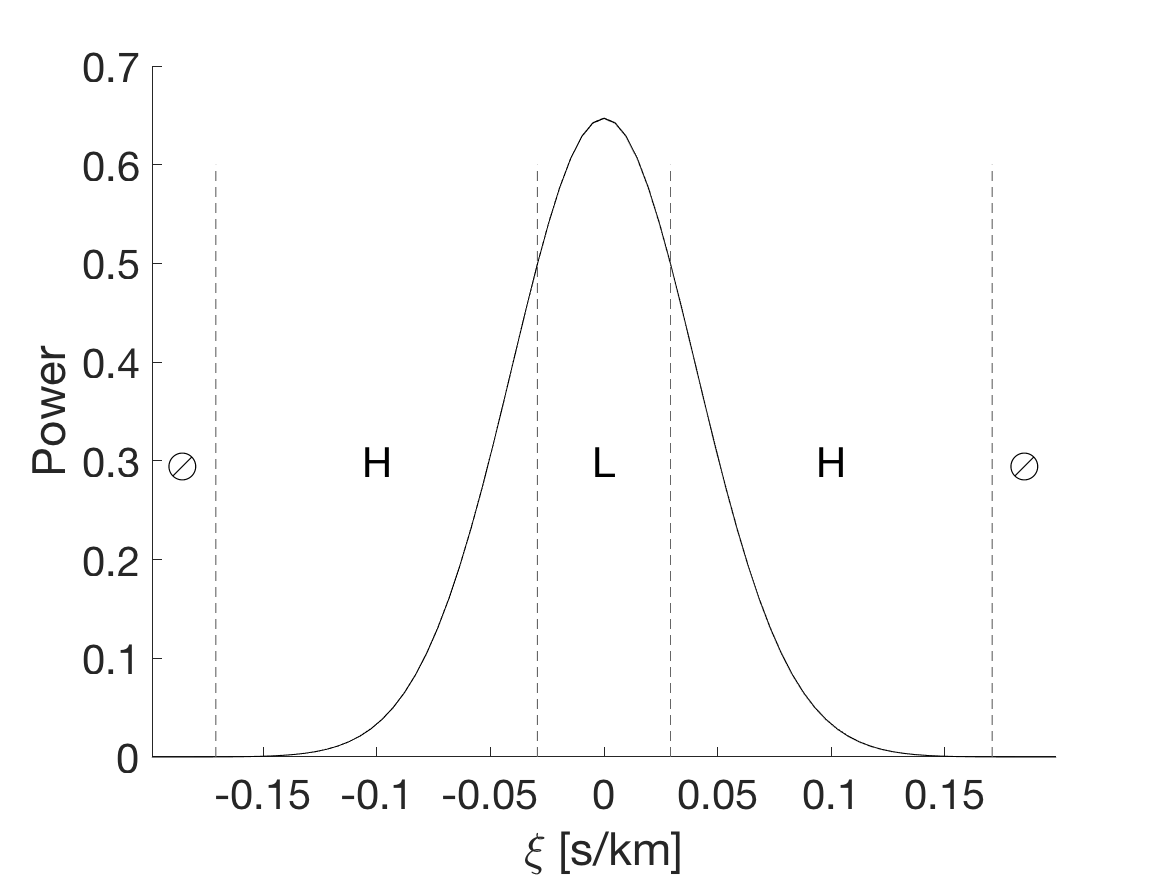
\includegraphics[width=\textwidth]{./Figures/Methods/LPD2-FT_power.png}
        \caption{Power spectrum (stacked)}
    \end{subfigure}
	~
    \begin{subfigure}[b]{0.49\textwidth}
        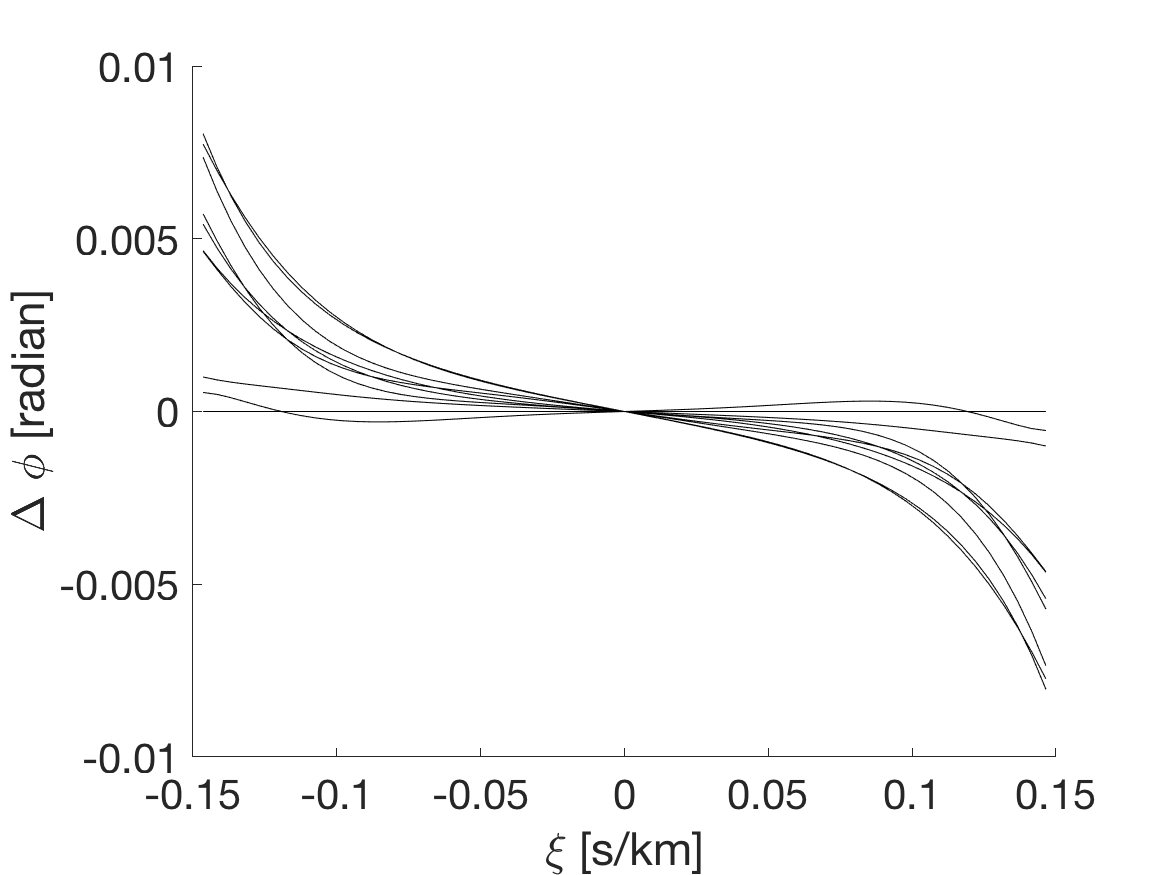
\includegraphics[width=\textwidth]{./Figures/Methods/LPD4-Relative_phase_angle.png}
        \caption{Differential phase spectrum}
        \label{fig:dps_LPD}
    \end{subfigure}	
    
    \caption[Fourier transform of deformed line profile]{Fourier transform of deformed line profile.}
\label{fig:FT_process_LPD}
\end{figure}    
%-------------

If we compare the differential phase spectra in Fig.~\ref{fig:FT_process} and Fig.~\ref{fig:FT_process_LPD},
it is quite obvious that the differential phase spectrum of a deformed line profile is no longer linear 
due to the $x_0$ dependency on $\xi$, as we discussed in \S~\ref{sec:LD_Theory}. Nevertheless, applying the 
local linear approximation will provide a radial velocity shift for that frequency range. We will primarily 
use the lower frequency range (from -0.06 to 0.06~(km/s)$^{-1}$ in this case) for the reasons that 
it is where information is mostly concentrated and that it is less noise-sensitive. 

We find, to our surprise, that $RV_\text{FT}$ is not only linearly correlated with $RV_\text{Gaussian}$, 
but also comes with a non-unity slope $k \sim 0.84$ (Fig.~\ref{fig:FT_vs_Gaussian}). 
The non-zero slope indicates without line shift, the intrinsic line deformation alone
disguises itself so well that even analysing the radial velocity shift by frequency has its limitations.
However, it does turn out that frequency analysis in the lower frequency bases 
are less sensitive to line deformation. In this particular circumstance, the region that we study has a frequency modulation of 
$\mid\xi\mid < 0.06$ (km/s)$^{-1}$, which is equivalent to oscillations of wavelengths $\lambda = 1/\mid\xi\mid > 16$ km/s.
These are indeed lower frequency modes less effectively modulated by the higher frequency deformations, as shown in the 
differential line profile in Fig.~\ref{fig:ld_dlp}. In addition, the slope $k$ will change depending on the 
frequency range in which the linear regression model is applied. 
For example, if we select the higher frequency range in the differential phase spectrum, we will 
expect larger $RV_\text{FT}$ and hence a larger $k$ in general. 

%-------------
\begin{figure}[htbp]
\centering
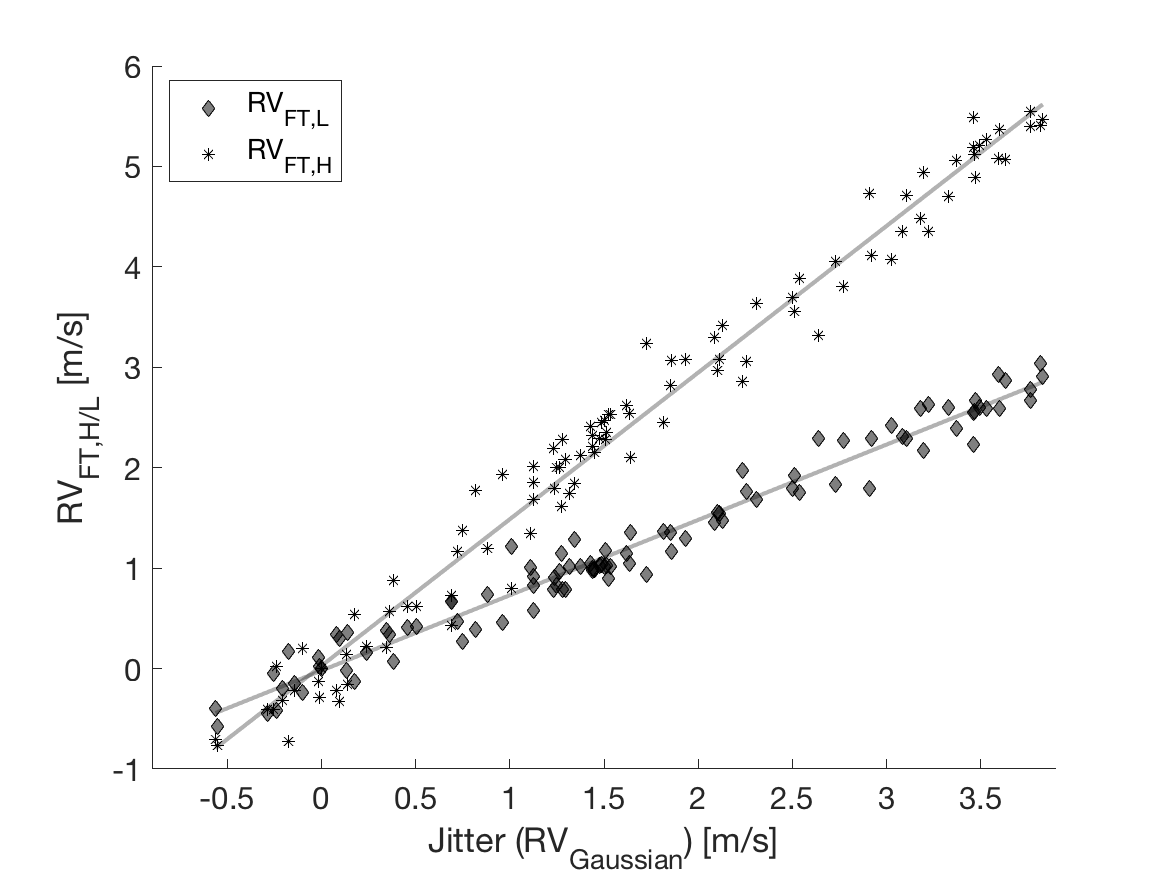
\includegraphics[width = 0.8 \linewidth]
{./Figures/Methods/5-JITTER_ONLY_1.png}
\caption[Fourier transform in response to line deformation]
{$RV_\text{FT} \sim k \cdot RV_\text{Gaussian}~(k<1)$}
\label{fig:FT_vs_Gaussian}
\end{figure} 
%-------------


\subsection{Jitter model}

We have learnt in \S~\ref{ch:FT_line_shift} that $RV_\text{FT}$ and $RV_\text{Gaussian}$
demonstrate basically the same response to radial velocity shifts. 
We have also learnt in this section (\S~\ref{sec:FT_ld}) that $RV_\text{FT}$ in the lower frequency range
is less sensitive to line deformation than $RV_\text{Gaussian}$, scaled by the factor $k$. 
Therefore, we write the following measurable quantities -- $RV_\text{FT}$ and $RV_\text{Gaussian}$ --
as the sum of corresponding contributions from the planet(s) and stellar variability (a.k.a jitter):
\begin{equation}
	RV_\text{Gaussian} = RV_\text{planet} + RV_\text{jitter}
\label{eq:RV_Gaussian}
\end{equation}
and
\begin{equation}
	RV_\text{FT} = RV_\text{planet} + k \cdot RV_\text{jitter}. 
\label{eq:RV_FT}
\end{equation}
Subtracting one from the other cancels out $RV_\text{planet}$ and gives
\begin{equation}
	\Delta RV = (1-k) \cdot RV_\text{jitter}
\end{equation}
where $\Delta RV = RV_\text{Gaussian} - RV_\text{FT}$. Rearranging yields 
\begin{equation}
	RV_\text{jitter} = \alpha \cdot \Delta RV
\label{eq:jitter_model}
\end{equation}
where $\alpha = 1/(1-k)$ is a scaling factor.  


\subsection{Sanity check}
\label{sec:check}

We will again perform a sanity check to see if we could correctly recover the jitter
based on our jitter model (Eq.~\ref{eq:jitter_model}). 

To start with, we generate 200 deformed line profiles (in the form of cross-correlation functions) with SOAP~2.0.
All the configurations are the same as \S\ref{sec:Simulations} except that they are evenly sampled throughout two
rotation periods. The jitter amplitude is roughly 2 m/s. 
In addition, each line profile is further shifted by an amount $RV_\text{planet}$, of which the amplitude
\begin{equation*}
	A_\text{planet} = 2~\text{m/s}
\end{equation*}
and the planetary orbital frequency to stellar rotation frequency ratio
\begin{equation*}
	\frac{\nu_\text{orb}}{\nu_\text{rot}} = \frac{P_\text{rot}}{P_\text{orb}} = 0.7.
\end{equation*}
In fact, the $RV_\text{planet}$ configuration shouldn't matter much 
because it will be mostly cancelled out in the jitter model. We then obtain two sets of radial velocities: 
$RV_\text{Gaussian}$ and $RV_\text{FT}$, as seen in the upper panel of Fig.~\ref{fig:PLANET_AND_JITTER}. 
As we know the amount of input jitter in our simulation, we simply scale up $\Delta RV$ by a parameter $\alpha$
to match the input jitter (dashed line in middle panel). 
The jitter model (black dots in middle panel) becomes more scattered as $\alpha \gg 1$.  
As a result, a moving average modulated by a Gaussian kernel is implemented to smooth out the data (solid line 
in middle panel).

To comment on the performance, we compare the rms of the input jitter $rms_\text{jitter}$
and the rms of the residual between the input jitter and the model jitter $rms_\text{residual}$. 
The former can be treated as the scatter after fitting the correct planet(s) without jitter correction, 
while the latter treated as the scatter after the additional jitter is removed.
The rms is reduced from $rms_\text{jitter} = 1.22$~m/s to $rms_\text{residual} = 0.70$~m/s,
which is crucial in enhancing the detection of planets with radial velocities of sub-m/s amplitudes. 
However, we should also note that there are systematic differences between the input jitter and our model jitter
(i.e. the residual sorts of repeats itself in the two stellar rotation periods). We should be aware that 
while removing the stellar variability contribution from the data, it may also add in some remnant features. 

%-------------
\begin{figure}[tbp]
\centering
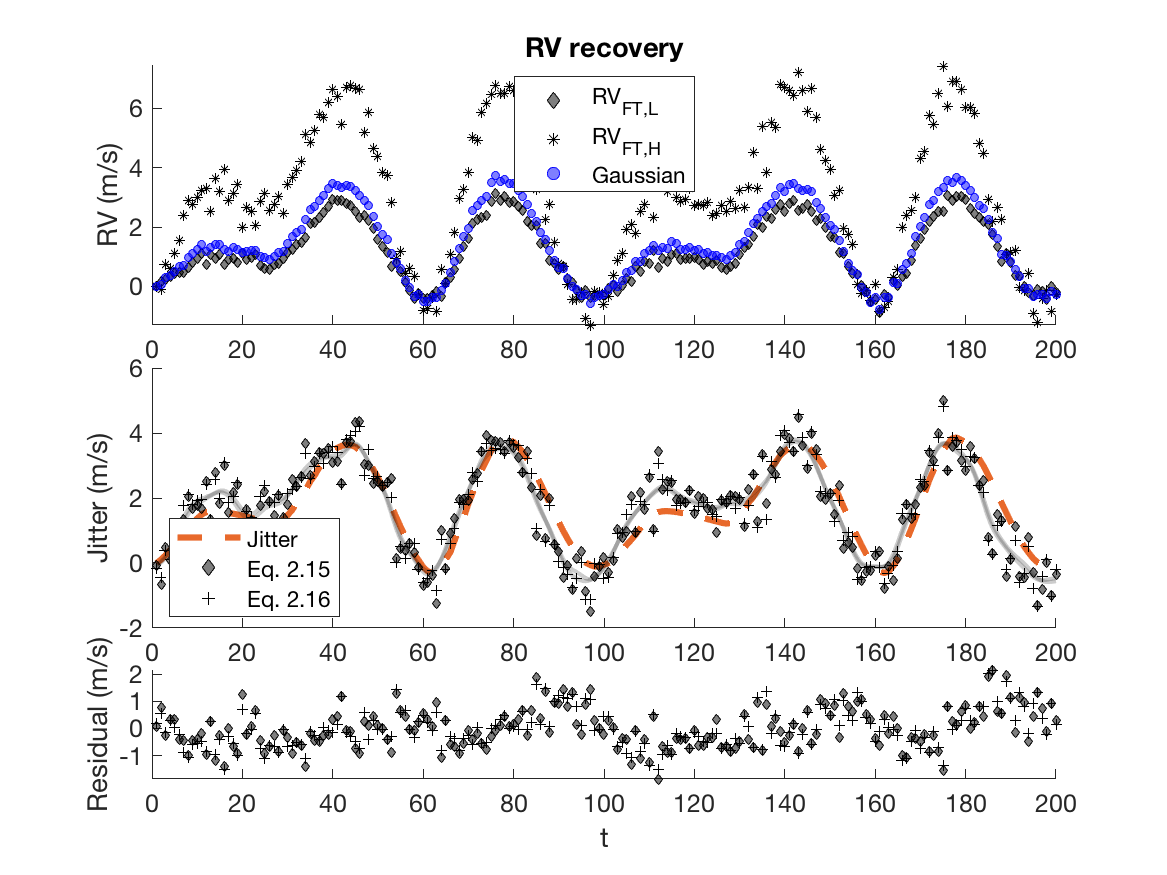
\includegraphics[width = 0.99 \linewidth]
{./Figures/Methods/5-PLANET_AND_JITTER.png}
\caption[Jitter model]
{Construct jitter model from simulation data.}
\label{fig:PLANET_AND_JITTER}
\end{figure} 
%-------------


\subsection{End-to-end Simulations}

Unless we are sure of a null-planetary system where $RV_\text{planet} = 0$ and
from Eq.~\ref{eq:RV_Gaussian} and Eq.~\ref{eq:RV_FT} we obtain
\begin{equation}
	k = RV_\text{jitter} / RV_\text{Gaussian},
\end{equation} 
normally $k$ cannot be directly calculated, so neither can $\alpha$ be.
However, we could substitute the jitter model (Eq.~\ref{eq:jitter_model}) into Eq.~\ref{eq:RV_Gaussian}, such that
\begin{equation}
	RV_\text{Gaussian} = RV_\text{planet} + \alpha \cdot \Delta RV
\label{eq:RV_fit}
\end{equation}
where $RV_\text{planet}$ is parametrised by Keplerian orbit(s) and both $RV_\text{Gaussian}$ and $\Delta RV$ 
are measurable. 

The tests are divided into two groups for comparison:
\begin{enumerate}
	\item Fit $RV_\text{Gaussian}$ by Keplerian orbit alone;
	\item Fit $RV_\text{Gaussian}$ by Keplerian orbit + jitter model (i.e. $\alpha \cdot \Delta RV$).
\end{enumerate}
The injected planet has the same parameter settings as in \S\ref{sec:check}, i.e. circular orbit with amplitude $A = 2$~m/s,
orbital frequency ratio $\nu = 0.7$ and initial phase $\omega = 1$~rad. We will compare which group recovers the 
planet parameters better. 

To better simulate the real observations, 40 data samples out of 200 from the two rotation periods are randomly selected.  
The fitting is achieved by running MCMC to maximise the log-likelihood function
given the model. For the simulation, each radial velocity data is equally weighted (as they have the same S/N). 
It is defined if the input parameter lies within $1\sigma$ errorbar of the output parameter, it counts as a 
successful detection. 

For demonstration, we show one of the outputs in corner plots (Fig.~\ref{fig:Corner}) and the corresponding 
radial velocity fitting (Fig.~\ref{fig:Planet_recovery}). The corner plot visually shows the how the walkers explore the parameter 
space and their distribution. The histogram gives an example explaining how a ``successful detection" is qualified. 
The radial velocity fitting plot demonstrates an example that implementing the jitter model effectively 
accounts for the spurious signals in the raw radial velocity data, reducing the rms from 1.14~m/s to 0.55~m/s. 

%-------------
\begin{figure}[tbp]
\centering
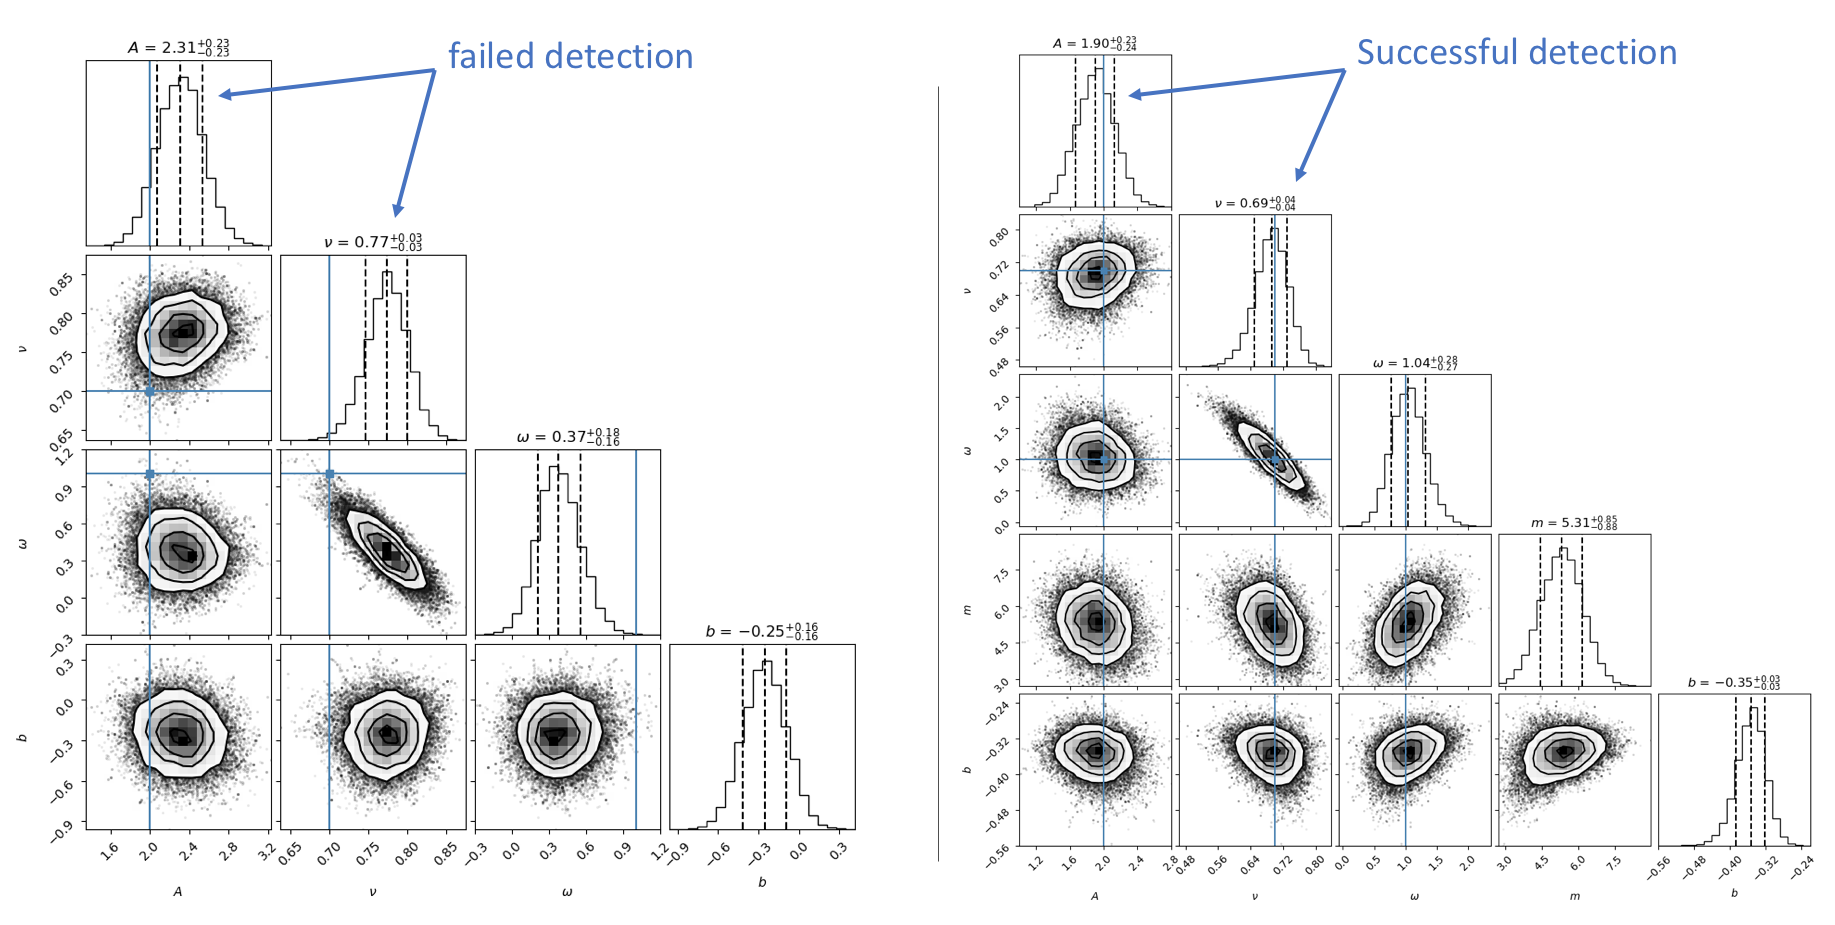
\includegraphics[width = 0.99 \linewidth]
{./Figures/Methods/Corner.png}
\caption[Corner plots of MCMC]
{Corner plots of MCMC. Theses are two examples of the output of MCMC: no jitter correction on the left and 
with jitter correction on the right. The input parameters are highlighted in the 
blue solid line. The three dashed lines of each histogram indicate the median and $1\sigma$ on both sides. On the 
left panel both blue lines of $A$ and $\nu$ are outside the $1\sigma$ region, therefore it counts as a ``failed detection";
on the right panel, it counts as a successful detection within $1\sigma$.}
\label{fig:Corner}
\end{figure} 
%-------------

%-------------
\begin{figure}[tbp]
\centering
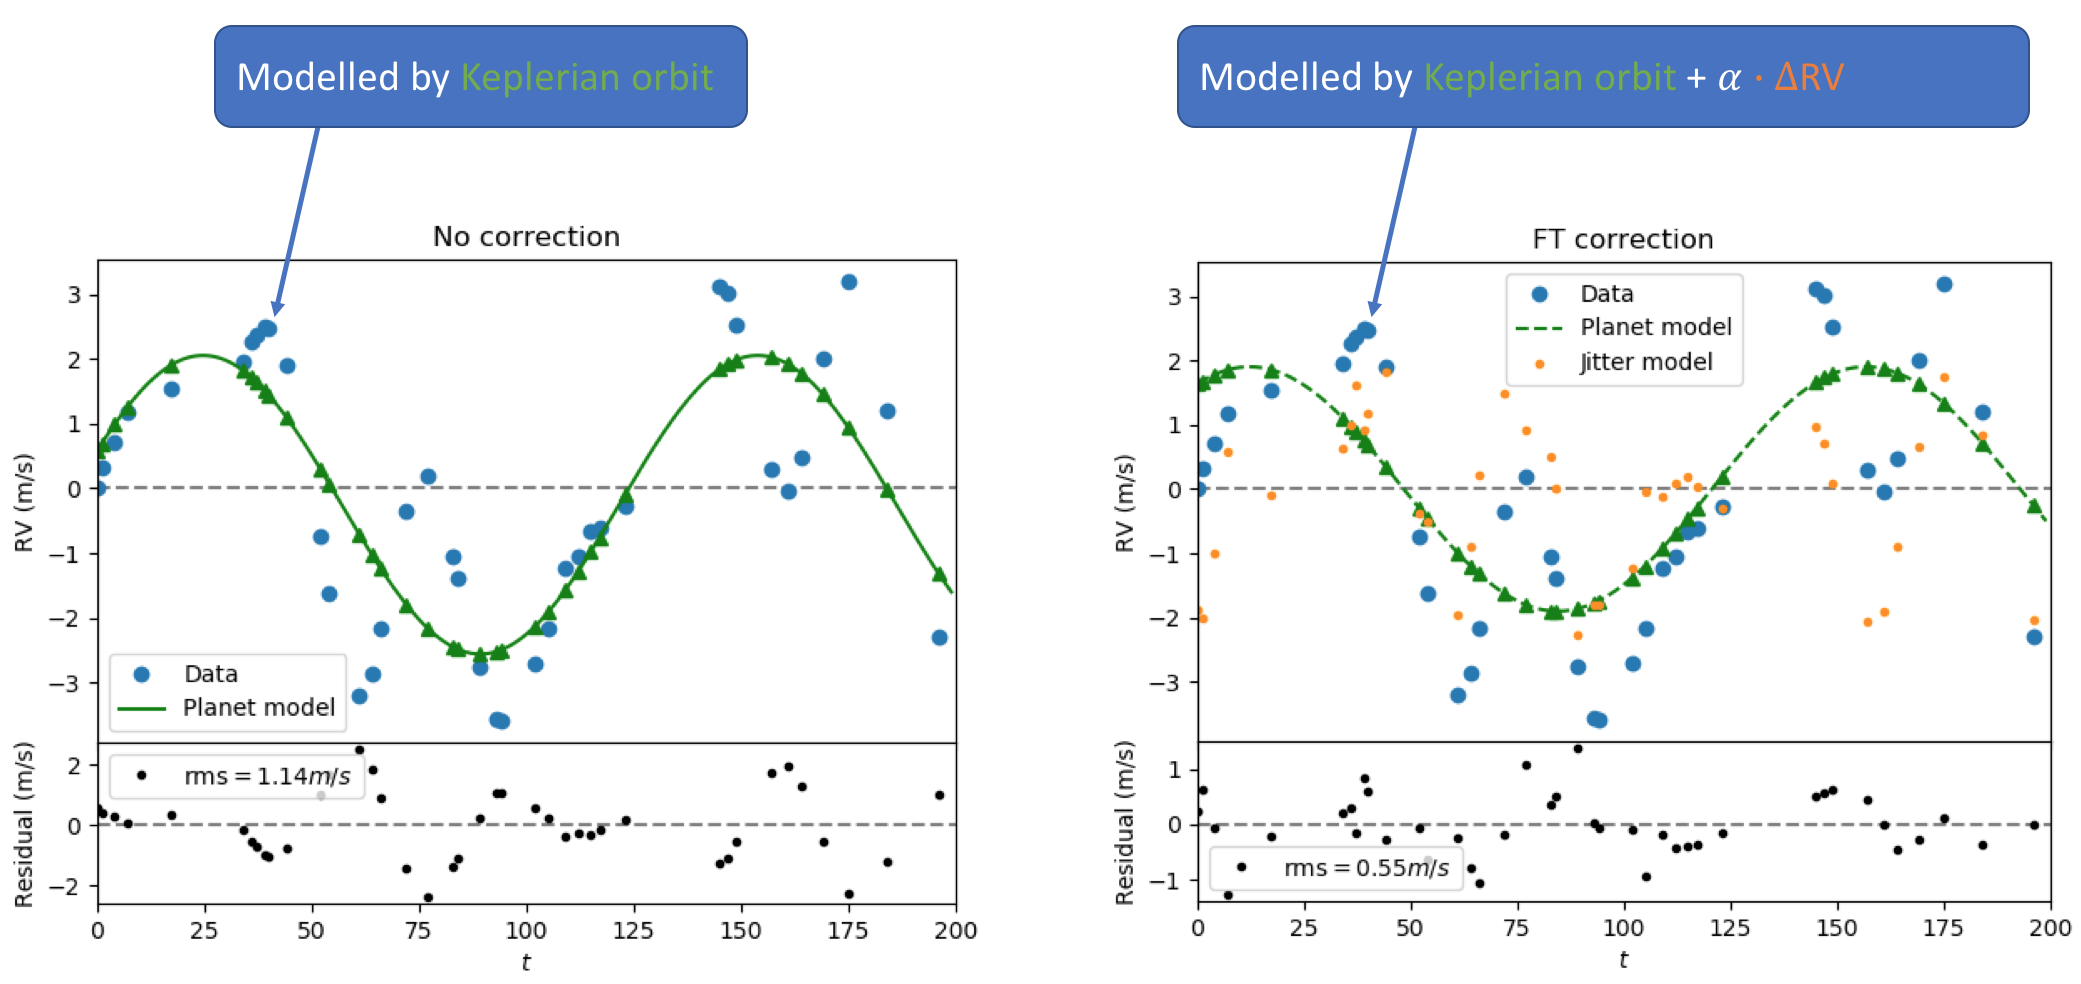
\includegraphics[width = 0.99 \linewidth]
{./Figures/Methods/Fitting.png}
\caption[Planet recovery]
{Radial velocity fitting. Theses are two fittings that comes out from the MCMC corner plots in Fig.~\ref{fig:Corner}. 
On the left panel without jitter correction, we can see that the input jitter increases the scatter of the raw radial 
velocities, resulting in an overestimated amplitude $A$; while on the right panel with jitter correction, the additional 
input jitter is accounted for by the jitter model.}
\label{fig:Planet_recovery}
\end{figure} 
%-------------

In the end, we run 100 trails for the end-to-end simulation. The random differences among these 100 trails come from:
\begin{itemize}
	\item photon noise given the S/N;
	\item randomly selected 40 samplings in the 200 line profiles.
\end{itemize}
It turns out that in $46\%$ of the 100 trails are successful detections for both $A$ and $\nu$ when we 
apply the jitter correction model, while this percentage is only $11\%$ without jitter correction. 
In more detail, Fig.~\ref{fig:FT_Statistics} shows that with jitter correction (in red), both of the amplitude and 
orbital frequency ratio tend to be underestimated, which is shown opposite for the results without correction (in blue). 
Moreover, the jitter corrected parameters are better constrained (i.e. with narrower distributions) and 
performs much better in $\nu$ than without correction. While it is tempting to say the correct answer is more likely in between
the results from these two fittings, we would need more tests to conclude. 

%-------------
\begin{figure}[tbp]	
    \begin{subfigure}[b]{0.49\textwidth}
        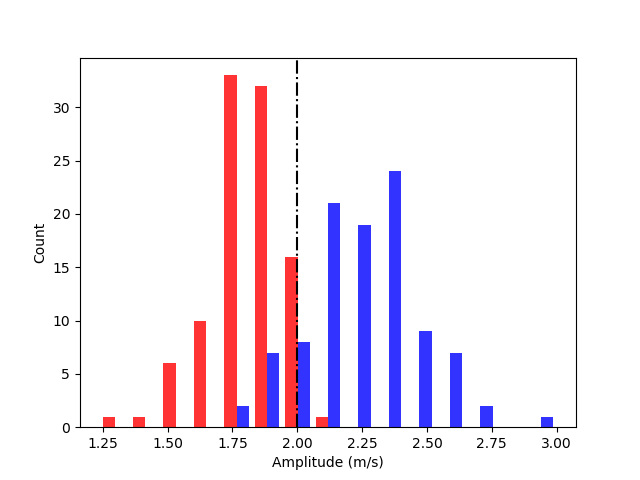
\includegraphics[width=\textwidth]{./Figures/Methods/Histogram_1.png}
        \caption{}
    \end{subfigure}
	~
    \begin{subfigure}[b]{0.49\textwidth}
        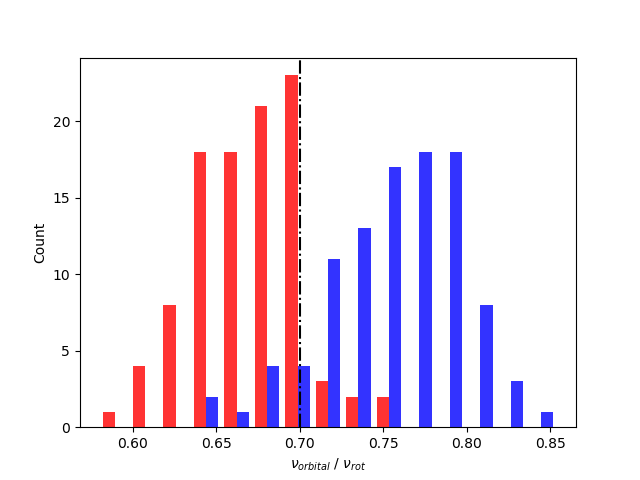
\includegraphics[width=\textwidth]{./Figures/Methods/Histogram_2.png}
        \caption{}
    \end{subfigure}	
    
    \caption[Distribution of recovered parameters]
    {Distribution of recovered parameters. The red are results of jitter correction by Fourier transform; 
    The blue are results of no jitter correction.}
\label{fig:FT_Statistics}
\end{figure}    
%-------------


%----------------------------------------------------------------------------------------
\section{Fourier transform with real observations}
\label{\thesection}
\label{sec:observation}

\subsection{HD189733: Rossiter–McLaughlin effect as jitter}

HD189733 is a well studied binary star system. The main star HD189733~A is known to host a gas giant
exoplanet HD189733~b, first detected by transits (reference...) and later by Doppler spectroscopy (references...). 
It was also the first exoplanet transit observed in X-ray (references...). 

We choose this target for the following reasons:
\begin{itemize}
	\item The exoplanet is well confirmed;
	\item The host star is bright enough: $m_v=7.66$
	\item The gas giant causes a prominent apparent radial velocity while it transits ($\sim 40$~m/s)
	due to Rossiter–McLaughlin effect.
\end{itemize}

%-------------
\begin{figure}[tbp]
\centering
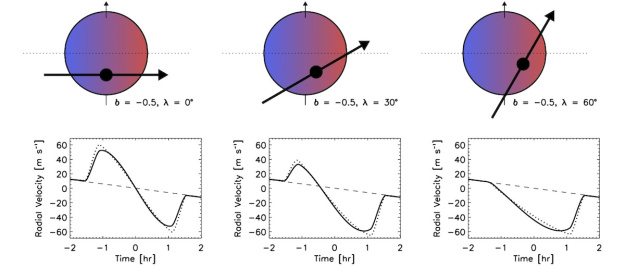
\includegraphics[width = 0.80 \linewidth]
{./Figures/Methods/rmeffect.jpg}
\caption[Demo: Rossiter–McLaughlin effect]
{Demo: Rossiter–McLaughlin effect (reference...). It is a apparent radial velocity
	change of the parent star due to an eclipsing binary (whether star or planet) that breaks the observed flux symmetry in the 
	stellar photosphere, resulting in imbalanced redshift and blueshift. It shows in this plot three different star-planet 
	alignments that causes three corresponding different shapes of radial velocity curve, and hence the radial velocity curve
	sheds information on the geometry of the alignment.}
\label{fig:rm-effect}
\end{figure} 
%-------------

We treat as if it were an ``active" star with one big dark starspot, as the Rossiter–McLaughlin effect 
causes the line profile deformed in a similar manner that a starspot would do (Fig.~\ref{fig:rm-effect}). 
We would see if our jitter model can account for the radial velocity variation from Rossiter–McLaughlin effect. 

The procedure is rather standardized. Both $RV_\text{Gaussian}$ and $RV_\text{FT}$ are calculated from the 
HARPS cross-correlation functions of the spectra. $\Delta RV = RV_\text{Gaussian} - RV_\text{FT}$ are then 
smoothed by a Gaussian filter (Fig.\ref{fig:hot_to_delta_rv}). The prototype of the Rossiter–McLaughlin
radial velocity curve is already identifiable in $\Delta RV$ of the lower panel. 

%-------------
\begin{figure}[tbp]
\centering
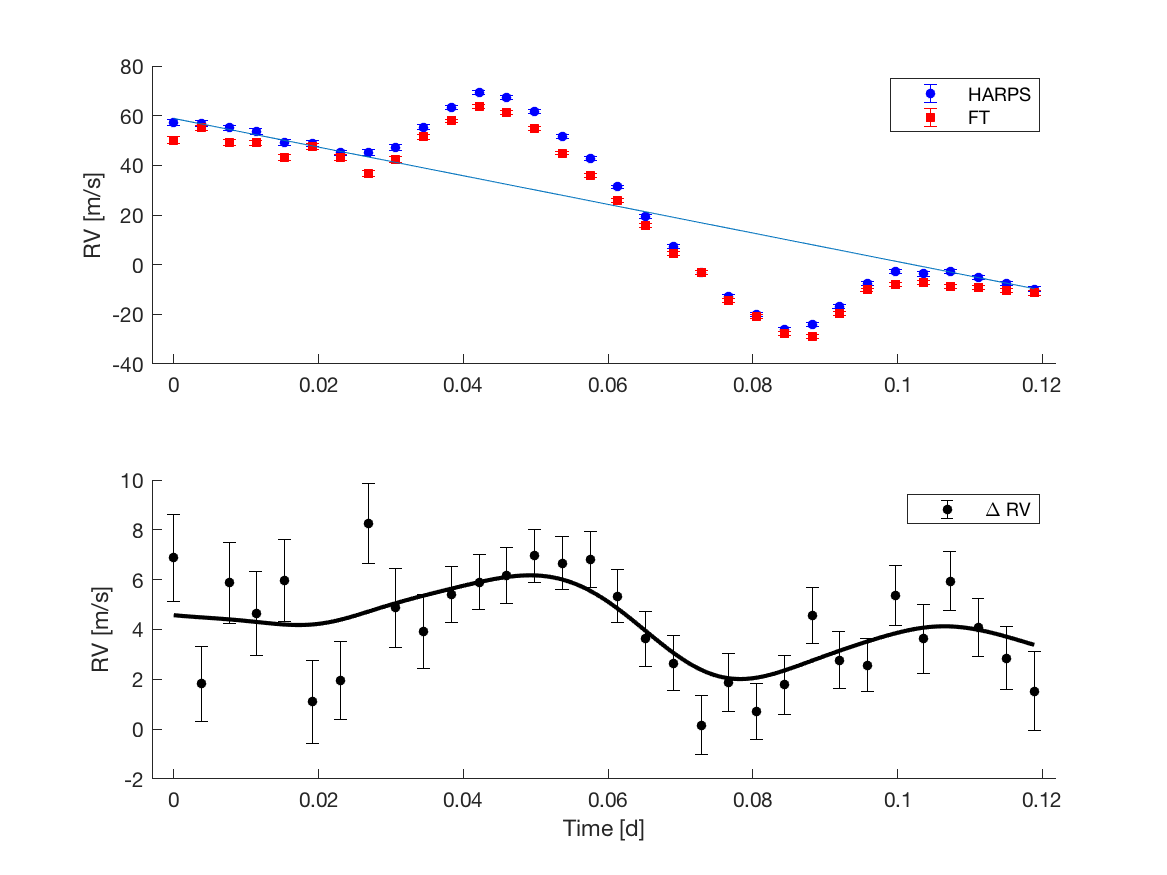
\includegraphics[width = 0.80 \linewidth]
{./Figures/Methods/8-Proto_jitter2.png}
\caption[From $RV_\text{Gaussian}$ and $RV_\text{FT}$ to $Delta RV$]
{From $RV_\text{Gaussian}$ and $RV_\text{FT}$ to $\Delta RV$. The scattered $\Delta RV$ are smoothed by applying 
a moving average with a Gaussian filter and  further weighted based on the size of errorbar.} 
\label{fig:hot_to_delta_rv}
\end{figure} 
%-------------

To extract the Rossiter–McLaughlin radial velocity curve, a linear trend is fitted to account for the 
other binary star. After the linear trend is removed, it is treated as jitter and modelled 
by $\alpha \cdot \Delta RV$ (Fig.~\ref{fig:rm_as_jitter}). 
Note that the errorbars of the jitter model also becomes a factor of $\alpha$ ($\alpha\gg 1$) larger; 
however, the model itself shows a descent approximation 
of the Rossiter–McLaughlin radial velocity curve. The peak of the ``jitter" is reduced from $\sim 40$~m/s to $\sim 10$~m/s. 

\paragraph{Remarks}
The effective length of the smoothing kernel should be carefully chosen. In this case, it's chosen most effective within 
roughly one neighbouring data point on both size. While mitigating the effect of noise (especially for relatively lower
S/N data outside the transits), to which the Fourier transform is sensitive, it also smears the drastic velocity 
change when the planet ingresses and egresses the stellar disk. To solve this awkward situation, an adaptive 
(i.e. S/N dependent) effective length of the smoothing kernel may be used. 

%-------------
\begin{figure}[tbp]
\centering
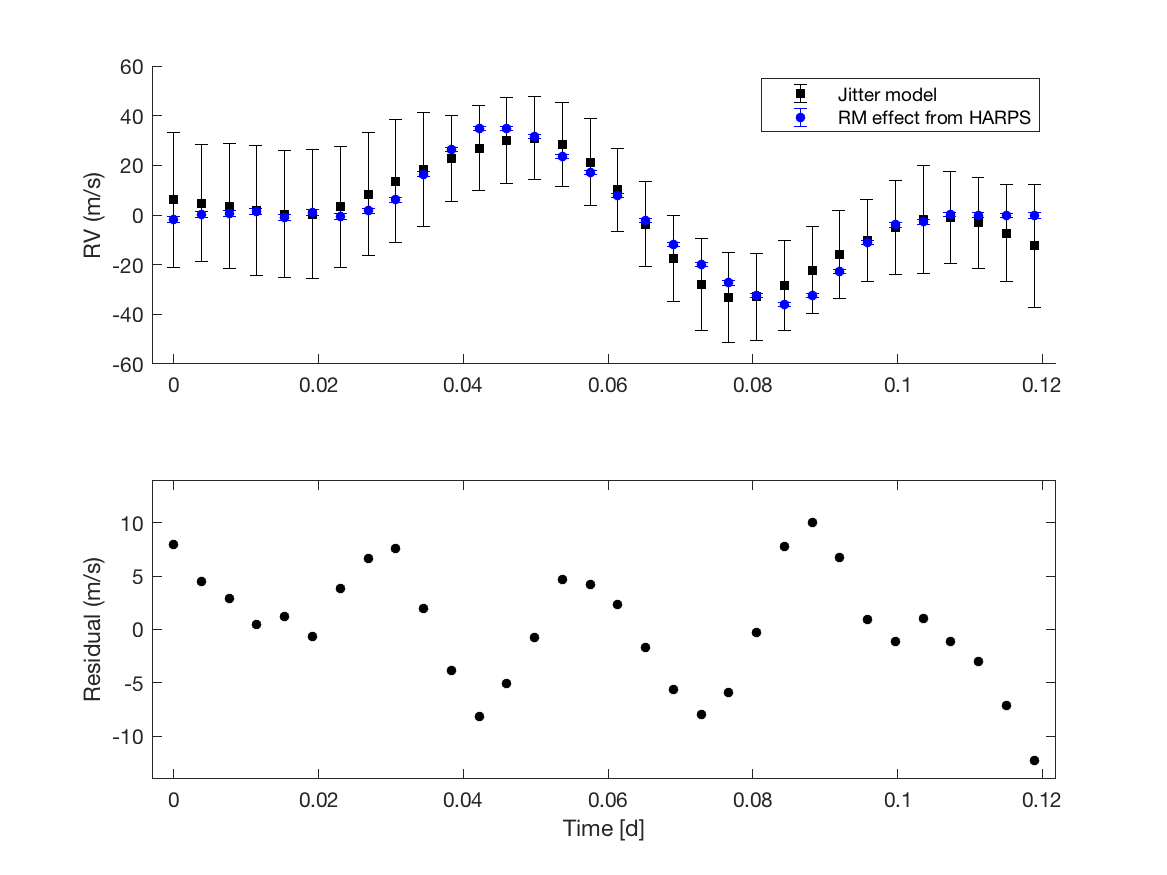
\includegraphics[width = 0.80 \linewidth]
{./Figures/Methods/9-RM_fit2.png}
\caption[Rossiter–McLaughlin effect as jitter]
{Rossiter–McLaughlin effect as jitter fitted with the jitter model.} 
\label{fig:rm_as_jitter}
\end{figure} 
%-------------

\subsection{Examples 2}

\subsection{Example 3}


%References like this: \cite{Selmeczi_07}


\FloatBarrier
A float barrier will stop figures from going beyond this point. They are handy to make sure they don't go into the next section.

%----------------------------------------------------------------------------------------
%\clearpage
\section{References}
\label{\thesection}
\vspace{-1.5cm}
\setstretch{1.0}
\bibliographystyle{unsrt}
\bibliography{Bibliography}
\setstretch{1.3}
